\section{Server Architecture}

The following is an overview about how the example chatbot has been created.
\\
Instead of covering all details, the focus here is to communicate the underlying concepts,
which are not unique to this specific chatbot and thereby enable others to apply similar patterns in their own development.
\\

\begin{figure}[h]
  \centering
  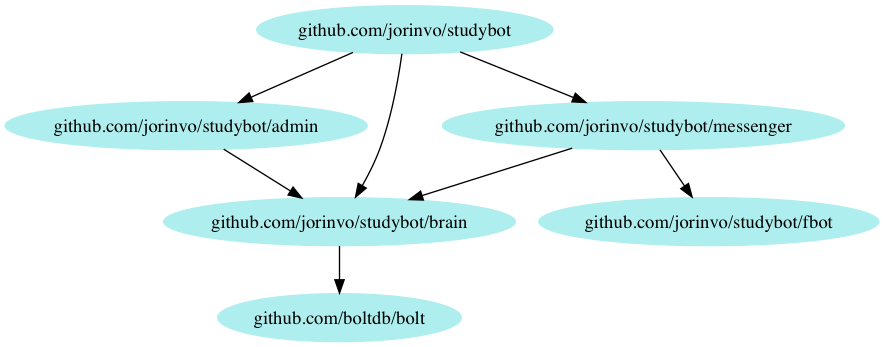
\includegraphics[width=0.8\textwidth]{images/internal-deps.png}
  \caption{Package dependency graph\footnotemark}
	\label{fig:internal-deps}
\end{figure}
\footnotetext{The graph has been created with \emph{godepgraph}\cite{godepgraph}}

There are numerous resources available today that demonstrate the development of chatbots.
However a majority of the existing material relies on specific services, frameworks or libraries for the implementation.
\\
The implementation of the example chatbot demonstrates all basics necessary for the creation of a chatbot
without relying on external tooling;
the code-base has no external dependencies, with the exception of a package for the database.
\\

The Graph in figure \ref{fig:internal-deps} shows the overall architecture of the chatbot.
\\
The \textbf{main} package handles only configuration, setup and tear-down.
It instantiates the data \emph{store} from package \textbf{brain}
and starts web servers listening on two separate ports for the packages \textbf{messenger} and \textbf{admin}.
\\

The \emph{store} has a connection to the database and it is responsible for all domain-specific business logic of \emph{Studybot}.
Both servers use the \emph{store} to fulfill their HTTP requests and they therefore depend on package \textbf{brain}.
\\
Package \textbf{admin} only provides functionality for internal use by the administrators of the chatbot;
one of its main responsibilities is to handle communication with Slack
for the in \ref{slackhook} on page \pageref{slackhook} mentioned feature.
\\

Package \textbf{messenger} is responsible for processing all events received from the Facebook Messenger platform.
\\

It relies on another package named \textbf{fbot},
which is a simple abstraction over the for this chatbot needed functionality of the Facebook Messenger platform.
Communication in this package happens via JSON over HTTP and since this is a custom package
specifically designed to be used in this chatbot, it only needs to support data types and parameters that are actually interesting to this product.
\\

\begin{figure}[h]
  \centering
  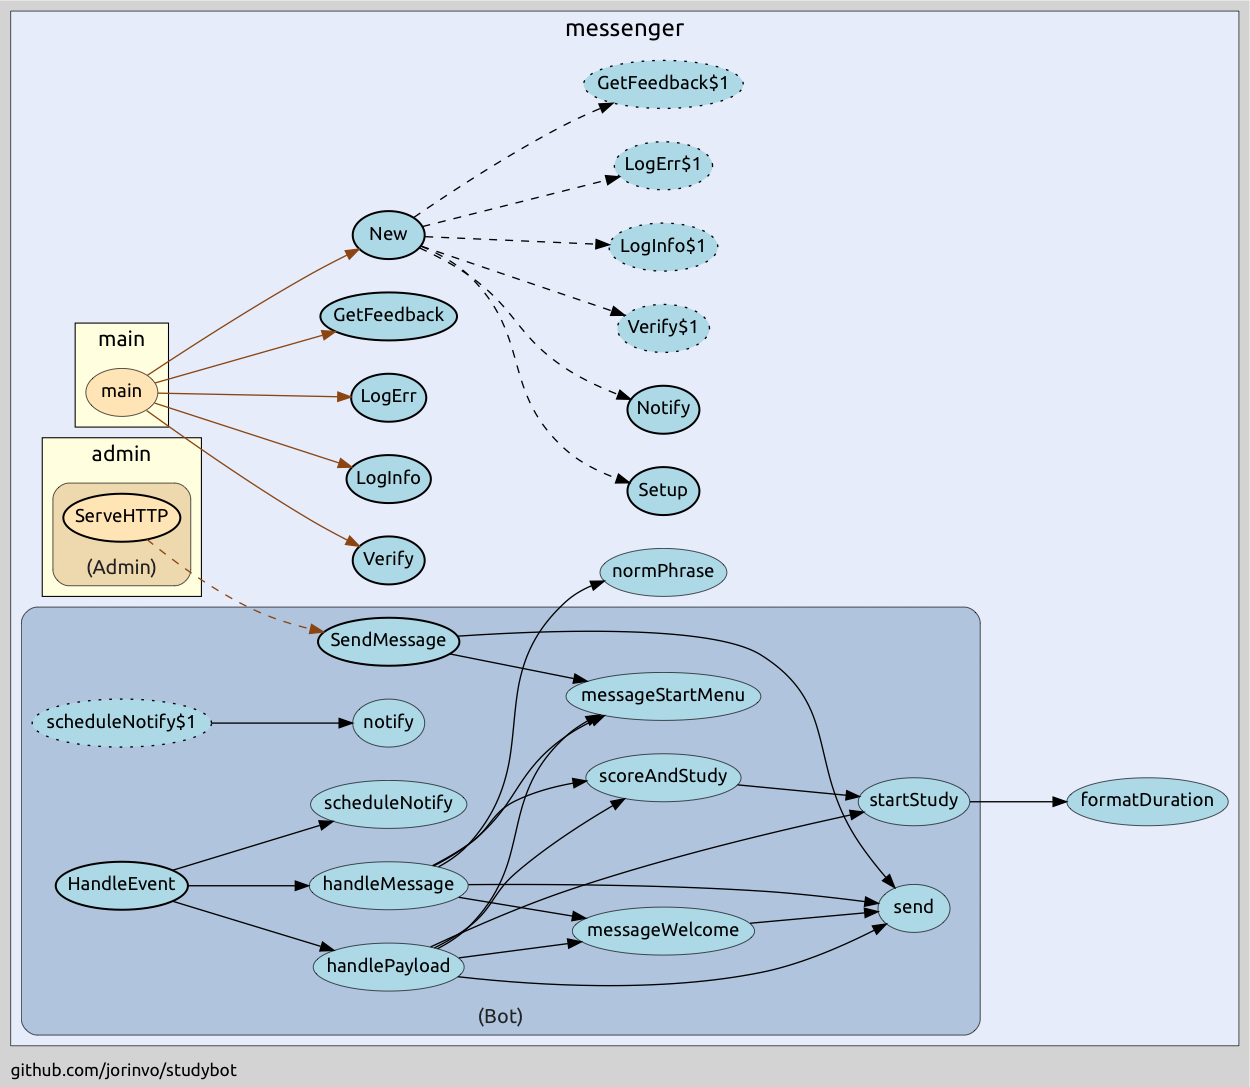
\includegraphics[width=0.8\textwidth]{images/call-graph-messenger.png}
	\caption{Call Graph of the messenger package\footnotemark}
	\label{fig:call-graph-messenger}
\end{figure}
\footnotetext{The visualization has been created with \emph{go-callvis}\cite{gocallvis}}


Most of the code-base and its architecture are structure the same way most other servers are organized,
the logic that is more specific to the development of a chatbot is mainly contained in the package \textbf{messenger}.
\\
Figure \ref{fig:call-graph-messenger} illustrates the behavior of this package,
but it should be noted that for brevity calls to the packages \textbf{brain} and \textbf{fbot} are not included in the graphic.
\\
The upper half of the graphic in \ref{fig:call-graph-messenger} shows function calls,
which are invoked from package \textbf{main} for initializing an instance of the type \emph{Bot}.
\\

The type \emph{Bot} provides functionality to handle events coming from the Facebook Messenger platform
and sending properly generated responses back to users.
\\
The function \emph{HandleEvent}, which can be seen in figure \ref{fig:call-graph-messenger},
is called by package \textbf{fbot} with every event the webhook receives,
and this is the main entry-point into the custom chatbot logic.
Depending on the type of the event,
\emph{HandleEvent} tracks whenever a user read a message,
or sends a message back to the user,
whereby it has to be differentiate between handling raw text messages
or handling the use of a predefined button and its action payload.
\\

In addition to directly responding to users,
\emph{HandleEvent} is also the source for scheduling the sending of notifications.
With every action of a user, the next time they receive a notification message needs to be rescheduled,
which happens in the call to the function \emph{scheduleNotify}.
The function in \ref{fig:call-graph-messenger} labeled as \emph{scheduleNotify\$1} is an anonymous callback function,
one for each user, that is called by the scheduled timer to send a message to the user.
\\

Further, it is visible in \ref{fig:call-graph-messenger},
that package \textbf{admin} can call a functioned named \emph{SendMessage} which belongs to the \emph{Bot} type.
This is used to send replies, that administrators created inside Slack, back to users,
since package \textbf{messenger} is the only package responsible for communicating with the Facebook Messenger platform.
\\

Limiting logic specific to the chosen platform, in this case Facebook Messenger,
makes it easier to adopt the chatbot to new platforms in the future.

% TODO
% Call graphs for the other packages can be found on \pageref{} in the appendix,
% and to further understand the generated documentation for all packages on \pageref{} can be consulted.
